%%%
%%%
\section{Assessing Anytime Performance}
\label{sec:anytime}
%\subsection{Benchmarking \irace and anytime assessment}

% and no statistically significantly differences can be found w.r.t. RE and \irace, using Friedman's non-parametric test with a confidence level of 98\%. %RE~(0.0022) and \irace~(0.0024) find high-performing architectures with similar probability, the performance of SMAC falls short~(0.0056). 
%Under this setup, \irace ranks last in the comparison to the remaining algorithms.
%Though \irace ranks last, our later discussion on alternative experimental setups willconfirm that \irace is a viable approach to \nasbench. 

As discussed in Section~\ref{sec:guidelines}, an assessment based solely on final quality excludes from the analysis the time required to achieve a given performance level. In this section, we perform an anytime comparison of all algorithms to investigate how their search dynamics differ. We also discuss the anytime effects of caching and of the variable-sized encoding. 


%, we compare the results based on the hypervolume indicator.
\subsection{Comparing Algorithms for Anytime Performance}
\begin{figure}[!t]
\centering
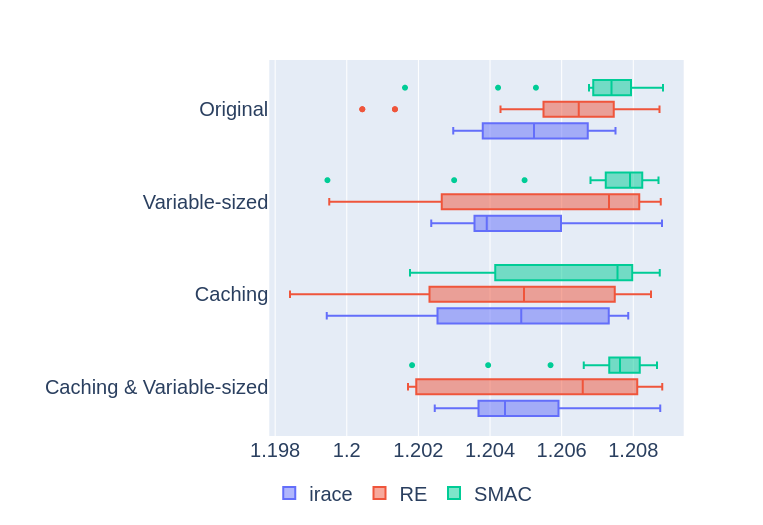
\includegraphics[width=0.9\linewidth, clip=true, trim=40px 20px 0 50px]{imgs/boxplots.png}
\caption{Boxplots of the hypervolume~($x$-axis) obtained in 20 runs from each of the algorithms selected, depicted in varying colors. Boxplots are grouped along the $y$-axis by the experimental setup adopted.}
\label{fig:boxplots}
\end{figure}

Figure~\ref{fig:boxplots} gives  boxplots of the hypervolume achieved by the algorithms in which runs are grouped by the experimental setup adopted. The smaller the value achieved, the better the anytime performance of the algorithm. The hypervolume indicator requires a reference point, and as traditionally done in the literature we use point $(2.1, 2.1)$. To do so, we initially normalize results to the $[1,2]$ range respectively using $[0,10^7]$ and $[0,1]$ as bounds for TPU time and mean test regret. 

For the original setup adopted in \nasbench, we observe intersections between the boxplots, though clearly SMAC outperforms \irace. This is confirmed by the rank sums given in Table~\ref{tab:rs-anytime}~(top), where SMAC is followed by RE and \irace ranks last. Interestingly, the variance in results increases in this order as well. The relative rankings observed for anytime performance contrast with the rankings observed for final quality in Table~\ref{tab:ecdf}~(top), where \irace ranked better than RE. The poor anytime performance of \irace is related to the budget set for each iteration, which is directly affected by the hyperparameters we configured for final-quality assessment. 
% no statistical significant difference can be found among all algorithms 
% %and no statistically significantly differences can be found w.r.t. RE and \irace, 
% using Friedman's non-parametric test with a confidence level of 98\%. 

\begin{table}[!t]
    \centering
    \caption{Rank sum (RS) analysis of hypervolumes grouped by experimental setup~(top) and algorithm~(bottom). O: original; VS: variable-sized; C: caching; CVS: caching \& variable-sized. Best-ranked levels are highlighted when statistically different different than others.}
    \label{tab:rs-anytime}
    \scalebox{0.85}{
    \begin{tabular}{r|r|r|r}
    \toprule
     O $\,$ & \bf{SMAC (30)}$\,$ & $\,$ \bf{RE (37)}$\,$  & $\,$ \irace (53) \\
    \midrule
    VS $\,$ & $\,$ \bf{SMAC (30)} & \bf{RE (40)}$\,$ & $\,$ \irace (50)  \\
    \midrule
    C $\,$ & $\,$ SMAC (32)$\,$ & RE (43)$\,$ & $\,$ \irace (45) \\
    \midrule
    CVS $\,$ & \bf{SMAC (30)}$\,$ & $\,$\bf{RE (43)}$\,$ & $\,$ \irace (47) \\
    \bottomrule
    \end{tabular}
    }\\[1em]
    \quad
    \scalebox{0.85}{
        \begin{tabular}{r|r|r|r|r}
        \toprule
            RE$\,$  & VS (47) & O (48) & CVS (49) & C (56)  \\
        \midrule
            \irace & O (45) & CVS (48) & C (52) & CVS (55) \\
        \midrule
            SMAC$\,$ & VS (43) & CVS (46) & O (54) & C (57)  \\
        \bottomrule
            \multicolumn{5}{c}{}\\[0.17cm]
        \end{tabular}
}\end{table}

We then compare the two best-performing algorithms, i.e., RE~(left) and SMAC~(right), with the help of empirical attainment function~(EAF) difference plots, given in Figure~\ref{fig:eaf-original}. As previously discussed, the $x$-axis depicts TPU time only, whereas the $y$-axis gives mean test regret. Dashed lines depict the 50\% attainment function from each algorithm, and differences depicted as shaded areas on either side of the plot indicate that the given algorithm presented a better performance at that point of the runs. 
RE is designed for this type of configuration scenario, favoring a quick intensification of the search. On the other hand, SMAC requires more TPU time to obtain a similar level of performance. This is the consequence of the evaluation strategy implemented by SMAC which, despite the low variability inherent to \nasbench, assumes the estimation of architecture performance to require several executions to be accurate. Hence, RE has a higher probability of obtaining best performance than SMAC with a lower TPU time budget, while for higher TPU times SMAC provides a better probability. If CPU-time were accounted for, however, the conclusions drawn from this comparison would likely be affected by the sequential nature of SMAC.
%These results highlight the benefits and pitfalls of the different search strategies implemented by SMAC and RE, providing a more accurate picture of their overall performance.

\begin{figure}[!t]
\centering
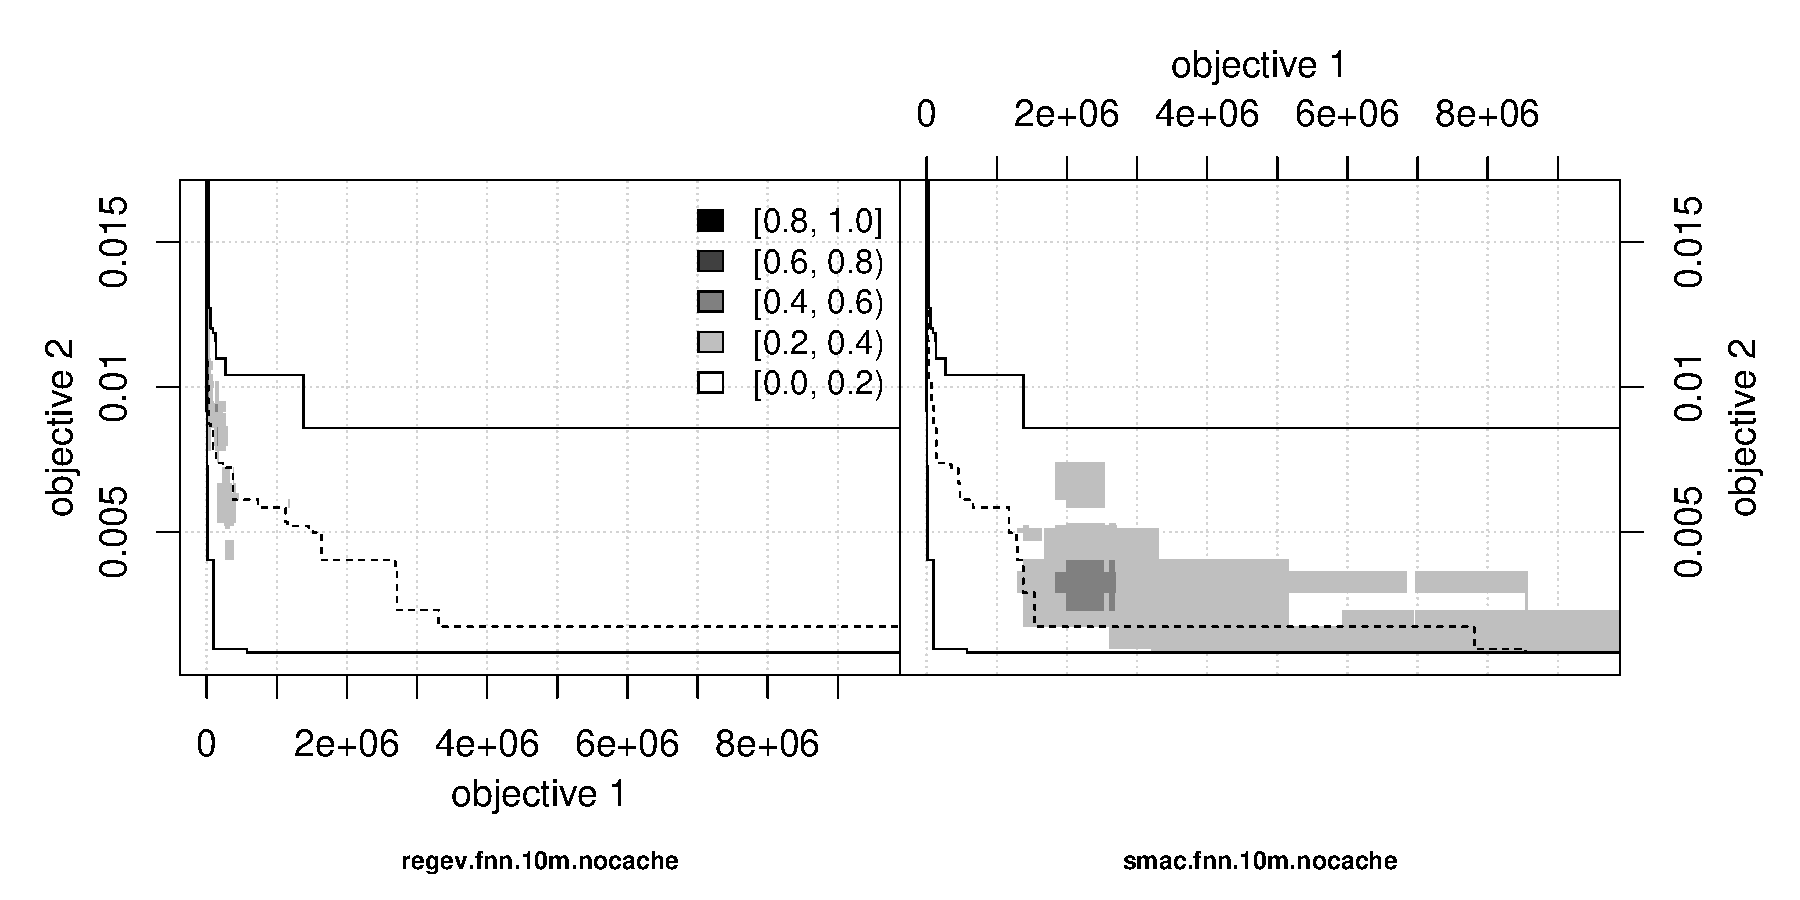
\includegraphics[width=\linewidth, clip=true, trim=45px 65px 85px 85px]{imgs/eaf-regev-smac-fnn-nocache.pdf}
\caption{Empirical attainment function~(EAF) difference plots comparing RE (left) and SMAC (right) run 20 times each. $x$-axis: TPU time; $y$-axis: mean test regret. %Dashed lines depict the 50\% attainment function from each algorithm. Differences depicted as shaded areas on either side of the plot indicate that the given algorithm presented a better performance at that point of the runs.
}
\label{fig:eaf-original}
\end{figure}

\subsection{Caching and Variable-Sized Encoding Effects}
The final-quality assessment discussed in the previous section showed that algorithm, variability degree, and solution encoding were interacting factors. Specifically, the only pattern observable in Table~\ref{tab:ecdf}~(bottom) referred to the caching strategy, which led to poor results for all algorithms when used with the fixed-size solution encoding. By contrast, Figure~\ref{fig:boxplots} shows that these alternative approaches affect most anytime performance as to the variance in the results. RE is the algorithm most affected, whereas SMAC is the least. Distribution shifts are also observed for all algorithms, though they vary as a function of the remaining factors. For SMAC and RE, the variable-sized encoding right-shifts the distributions, though a bit less in the presence of caching. Conversely, \irace presents its best anytime performance in the original \nasbench setup. 

The rank sum analysis given in Table~\ref{tab:rs-anytime} confirms these findings. On the top grouping, experimental setups do not alter the relative performance of the algorithms, though caching affects statistical significance due to the high variance in SMAC results discussed above. For the bottom grouping, rank sums for the different setups are very similar within each row, again due to the increased variance in results. As previously discussed, these conclusions should consider that all algorithms have been configured for final-quality optimization under the original setup. Yet, they further evidence the need for benchmarking NAS from an anytime performance perspective.

% A different pattern in boxplots is observed when we assess anytime performance for the variable-sized approach. For this setup, the variance in results is greatly increased for RE, whereas the distribution in SMAC is right-shifted. By contrast, the distribution of \irace presents a smaller As previously discussed for final-quality assessment, these results are consistent with our previous discussion on the benefits of ACs. \irace is unable to benefit here from this alternative setup. %Why??? I mean, who cares? :P
% Furthermore, though the increment in variance is much lower for \irace than for RE, the rank sum analysis given in Table~\ref{tab:ecdf}~(top) for this setup~(labeled VS) shows that RE is the least affected algorithm. This is likely explained by the changes in performances from the remaining algorithms and seed pairing, which the boxplots conceal. Yet, no statistically significant differences can be found among the algorithms once again.

% %The indicator is able to show clearly the differences performance between the algorithms. 
% % The hypervolume obtained by RE and \irace is significantly better than the obtained by SMAC (Wilcoxon test $\alpha=0.05$). While RE and \irace are close and the difference in their results is not significant.... \leslie{}{just inventing here...}

% Concerning anytime performance of caching evaluations, Figure~\ref{fig:boxplots} shows that caching indeed improves the performance of SMAC, as reported in the original \nasbench proposal. Yet, the remaining algorithms are negatively affected in variance and/or distribution shift. In the case of RE, we understand that an algorithm with strong convergence pressure benefits from variability to avoid early stagnation, and hence having longer to search does not help. As for \irace, having \leslie{}{the equivalent to} a single instance to work with greatly limits the benefits of seeing more configurations, as the statistical test used to discard races does not have enough evidence to work with. Though SMAC was also devised for multi-instance algorithm configuration, it is an extended version of an originally per-instance configurator, and hence it is better equipped to approach \nasbench. Nevertheless, the rank sum analysis provided in Table~\ref{tab:rs-anytime}~(top) for this setup~(labeled C) shows that all algorithms are considered statistically equivalent.

% If both caching and variable-sized encoding are considered at the same time, anytime results are a combination of the results seen for these individual factors. In more detail, SMAC improved its anytime performance when either caching or variable-sized encoding were adopted, so combined they lead SMAC to a significantly better performance than the remaining algorithms. \irace, especially, shows a performance deterioration even greater than RE. This is shown both in Figure~\ref{fig:boxplots} and Table~\ref{tab:rs-anytime}~(top), in which this setup is labeled CVS. The interactions between experimental design choices and algorithms are summarized in Table~\ref{tab:rs-anytime}~(bottom), where we see that RE is the algorithm least affected.